\documentclass[aspectratio=169,11pt]{beamer}

\usetheme{Singapore}
\usepackage[utf8]{inputenc}
\usepackage{amsmath}
\usepackage{amsfonts}
\usepackage{amssymb}
\usepackage{graphicx}
\usepackage{hyperref}
\usepackage{booktabs}
\usepackage{listings}
\usepackage{xcolor}
\usepackage{caption}
\usepackage{subcaption}


% Define the settings for codechunks
\definecolor{codegreen}{rgb}{0,0.6,0}
\definecolor{codegray}{rgb}{0.5,0.5,0.5}
\definecolor{codepurple}{rgb}{0.58,0,0.82}
\definecolor{backcolour}{rgb}{0.9,0.9,0.9}
\lstdefinestyle{mystyle}{
    backgroundcolor=\color{backcolour},   
    commentstyle=\color{codegreen},
    keywordstyle=\color{magenta},
    numberstyle=\tiny\color{codegray},
    stringstyle=\color{codepurple},
    basicstyle=\ttfamily\footnotesize,
    breakatwhitespace=false,         
    breaklines=true,                 
    captionpos=b,                    
    keepspaces=true,                 
    numbers=left,                    
    numbersep=5pt,                  
    showspaces=false,                
    showstringspaces=false,
    showtabs=false,                  
    tabsize=2
}
\lstset{style=mystyle}

% Setup the bibliography
\usepackage[style=authortitle,backend=bibtex]{biblatex}
\addbibresource{bibliography.bib}
\setbeamertemplate{bibliography item}[text]
\setbeamerfont{footnote}{size=\tiny}

% Allow footnotes with no number
\newcommand\blfootnote[1]{%
  \begingroup
  \renewcommand\thefootnote{}\footnote{#1}%
  \addtocounter{footnote}{-1}%
  \endgroup
}

% Allow section title slides
\AtBeginSection[]{
  \begin{frame}
  \vfill
  \centering
  \begin{beamercolorbox}[sep=8pt,center,shadow=true,rounded=true]{title}
    \usebeamerfont{title}\insertsectionhead\par%
  \end{beamercolorbox}
  \vfill
  \end{frame}
}

\author{Dr Stephen Pederson}
\title{Lecture 8: Enrichment Testing}
\subtitle{BIOINF3005/7160: Transcriptomics Applications}
%\setbeamercovered{transparent} 
\setbeamertemplate{navigation symbols}{} 
\logo{
	
\includegraphics[scale=0.3]{figures/UoA_logo_col_vert.png} 
} 
\institute{Bioinformatics Hub, \\The University of Adelaide} 
\date{May 11th, 2020} 
\subject{BIOINF3005/7160: Transcriptomics Applications} 


\begin{document}

\begin{frame}
\titlepage
\end{frame}

\begin{frame}
\footnotesize
\tableofcontents
\end{frame}

\section{Databases}

\begin{frame}{Introduction}

	\begin{itemize}
		\item Once we have obtained results from our analysis:
		\begin{itemize}
			\item How do we summarise the results for hundreds/thousands of genes?
		\end{itemize}
		\item We look for biological patterns
		\item How do we even define biological patterns?
		\item We can use pre-existing databases with defined terms
		\begin{itemize}
			\item GO, KEGG, Wiki Pathways, MSigDB, JASPAR etc
		\end{itemize}
		\item We obtain pre-defined \textbf{gene sets} and test for enrichment in our dataset
	\end{itemize}

\end{frame}

%\subsection{The Gene Ontology Database}

\begin{frame}{The Gene Ontology Database}

	\begin{itemize}
		\item The most commonly used resource for describing biology
		\begin{itemize}
			\item Also one of the most frustrating		
		\end{itemize}
		\item Has a restricted vocabulary for describing biological features $\implies$ GO Terms
		\item Multiple classification levels for assigning GO terms to genes
		\item The basic structure is as a Directed Acyclic Graph (DAG)
	\end{itemize}
	
\end{frame}

\begin{frame}{The Gene Ontology Database}

	\begin{center}
	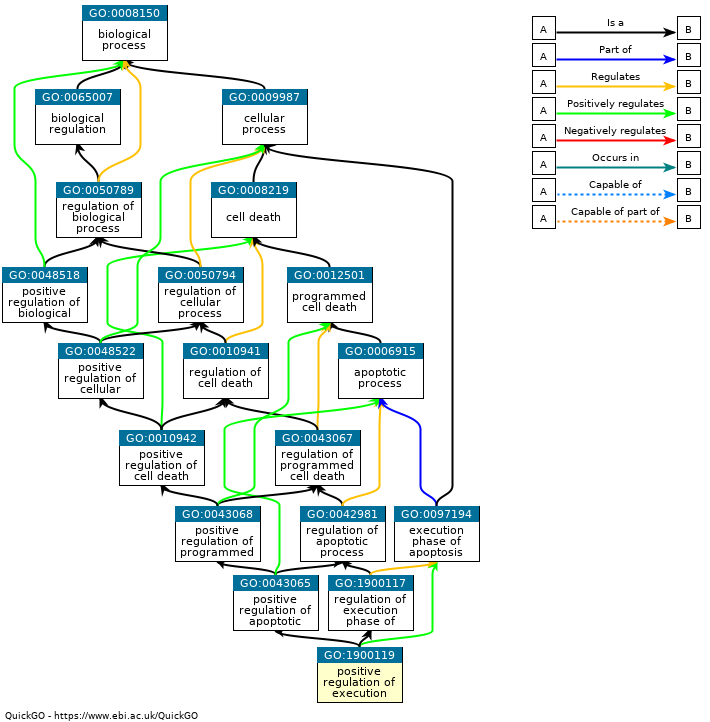
\includegraphics[width=0.4\textwidth]{figures/apoptosisDAG.png} 
	\end{center}


\end{frame}

\begin{frame}{The Gene Ontology Database}

The three Ontologies

	\begin{enumerate}
		\item \textbf{Molecular Function}: \textit{A molecular function is a process that can be carried out by the action of a single macromolecular machine, via direct physical interactions with other molecular entities}
		\pause
		\item \textbf{Cellular Component}: \textit{A cellular component is a location, relative to cellular compartments and structures, occupied by a macromolecular machine when it carries out a molecular function}
		\pause
		\item \textbf{Biological Process}: \textit{A biological process represents a specific objective that the organism is genetically “programmed” to achieve}
	\end{enumerate}
	
All definitions taken from Thomas (2017)\footfullcite{Thomas2017}

\end{frame}

\begin{frame}{The Gene Ontology Database}

	\begin{itemize}
		\item Each GO term belongs exclusively to one Ontology 
		\item Contains an ID, Name, Definition
		\item Browsing our term from the previous image: \url{https://www.ebi.ac.uk/QuickGO/term/GO:1900119}
	\end{itemize}

\end{frame}

\begin{frame}{The Gene Ontology Database}

	\begin{itemize}
		\item By definition, every term/node in each ontology inherits the properties of the parent node
		\item Each parent node contains several child terms directly beneath it 
		\begin{itemize}
			\item \url{http://amigo.geneontology.org/amigo/dd_browse}
		\end{itemize}
		\pause
		\item Each child node inherits the properties of it's parent node
		\item Children can have multiple parents
		\item Edges connect children to parents
	\end{itemize}

\end{frame}

\begin{frame}{The Gene Ontology Database}

	\begin{center}
	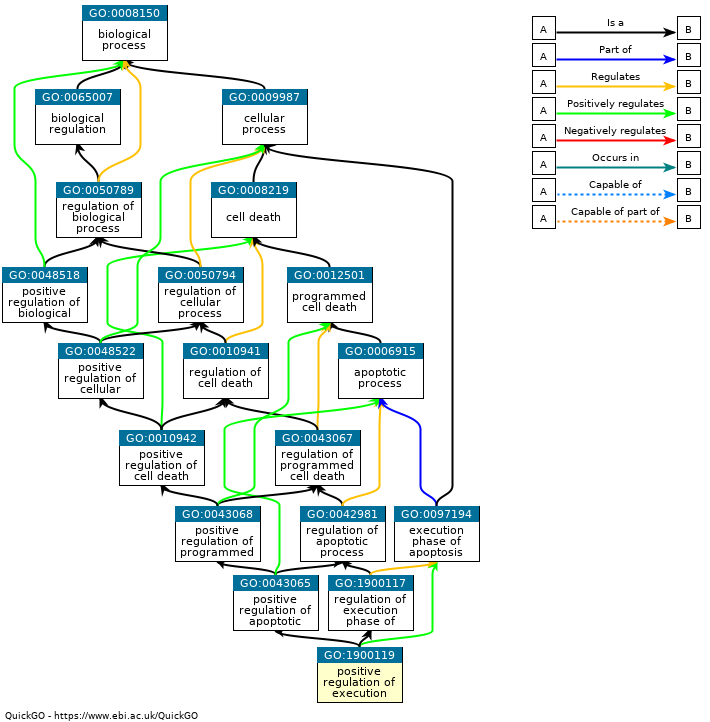
\includegraphics[width=0.4\textwidth]{figures/apoptosisDAG.png} 
	\end{center}


\end{frame}

\begin{frame}{The Gene Ontology Database}

	\begin{itemize}
		\item Once a term is defined, it can be assigned to a gene/protein
		\item We need evidence $\ldots$
		\begin{itemize}
			\item Multiple evidence codes are defined
			\item Each mapping of gene to term includes the level of evidence
			\item \url{http://geneontology.org/docs/guide-go-evidence-codes/}
		\end{itemize}
		\pause
		\item \textit{Evidence is species-specific}, but is often mapped across species
		\item IEA represents the lowest quality
		\begin{itemize}
			\item In non-model organisms, this might be all we have
		\end{itemize}
	\end{itemize}

\end{frame}

\begin{frame}{A Few Challenges with GO Annotation}

	\begin{enumerate}
		\item A set of specific terms are mapped to each gene
		\begin{itemize}
			\item Parent terms may or may not be
		\end{itemize}
		\item There is a high level of redundancy
		\begin{itemize}
			\item GO terms may overlap parent terms \textbf{significantly}
		\end{itemize}
		\item Visualisation for hundreds of GO terms from our analysis
		\begin{itemize}
			\item Can we cluster by semantic similarity
			\item Can we cluster by common membership (e.g. community detection)
		\end{itemize}
		\item Terms may also appear quite biologically abstract
	\end{enumerate}

\end{frame}

\begin{frame}{GO Visualisations}

	\begin{center}
	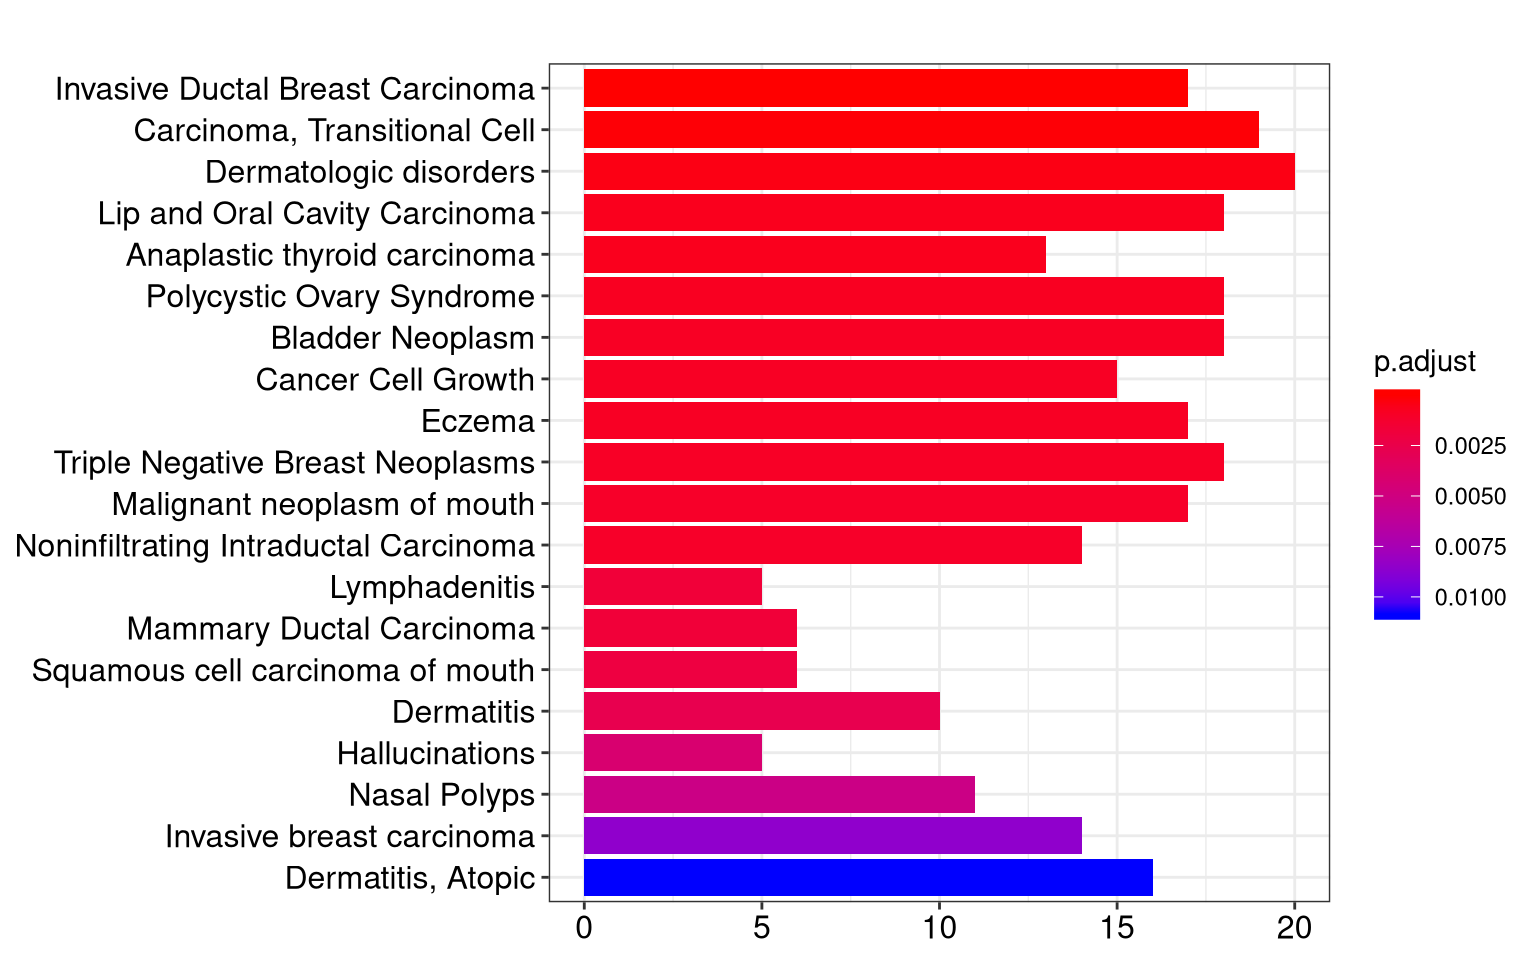
\includegraphics[width=0.6\textwidth]{figures/Barplot-1.png}
	\end{center}
	
\blfootnote{Image taken from clusterProfiler vignette \url{https://yulab-smu.github.io/clusterProfiler-book/chapter12.html}}

\end{frame}

\begin{frame}{GO Visualisations}

	\begin{center}
	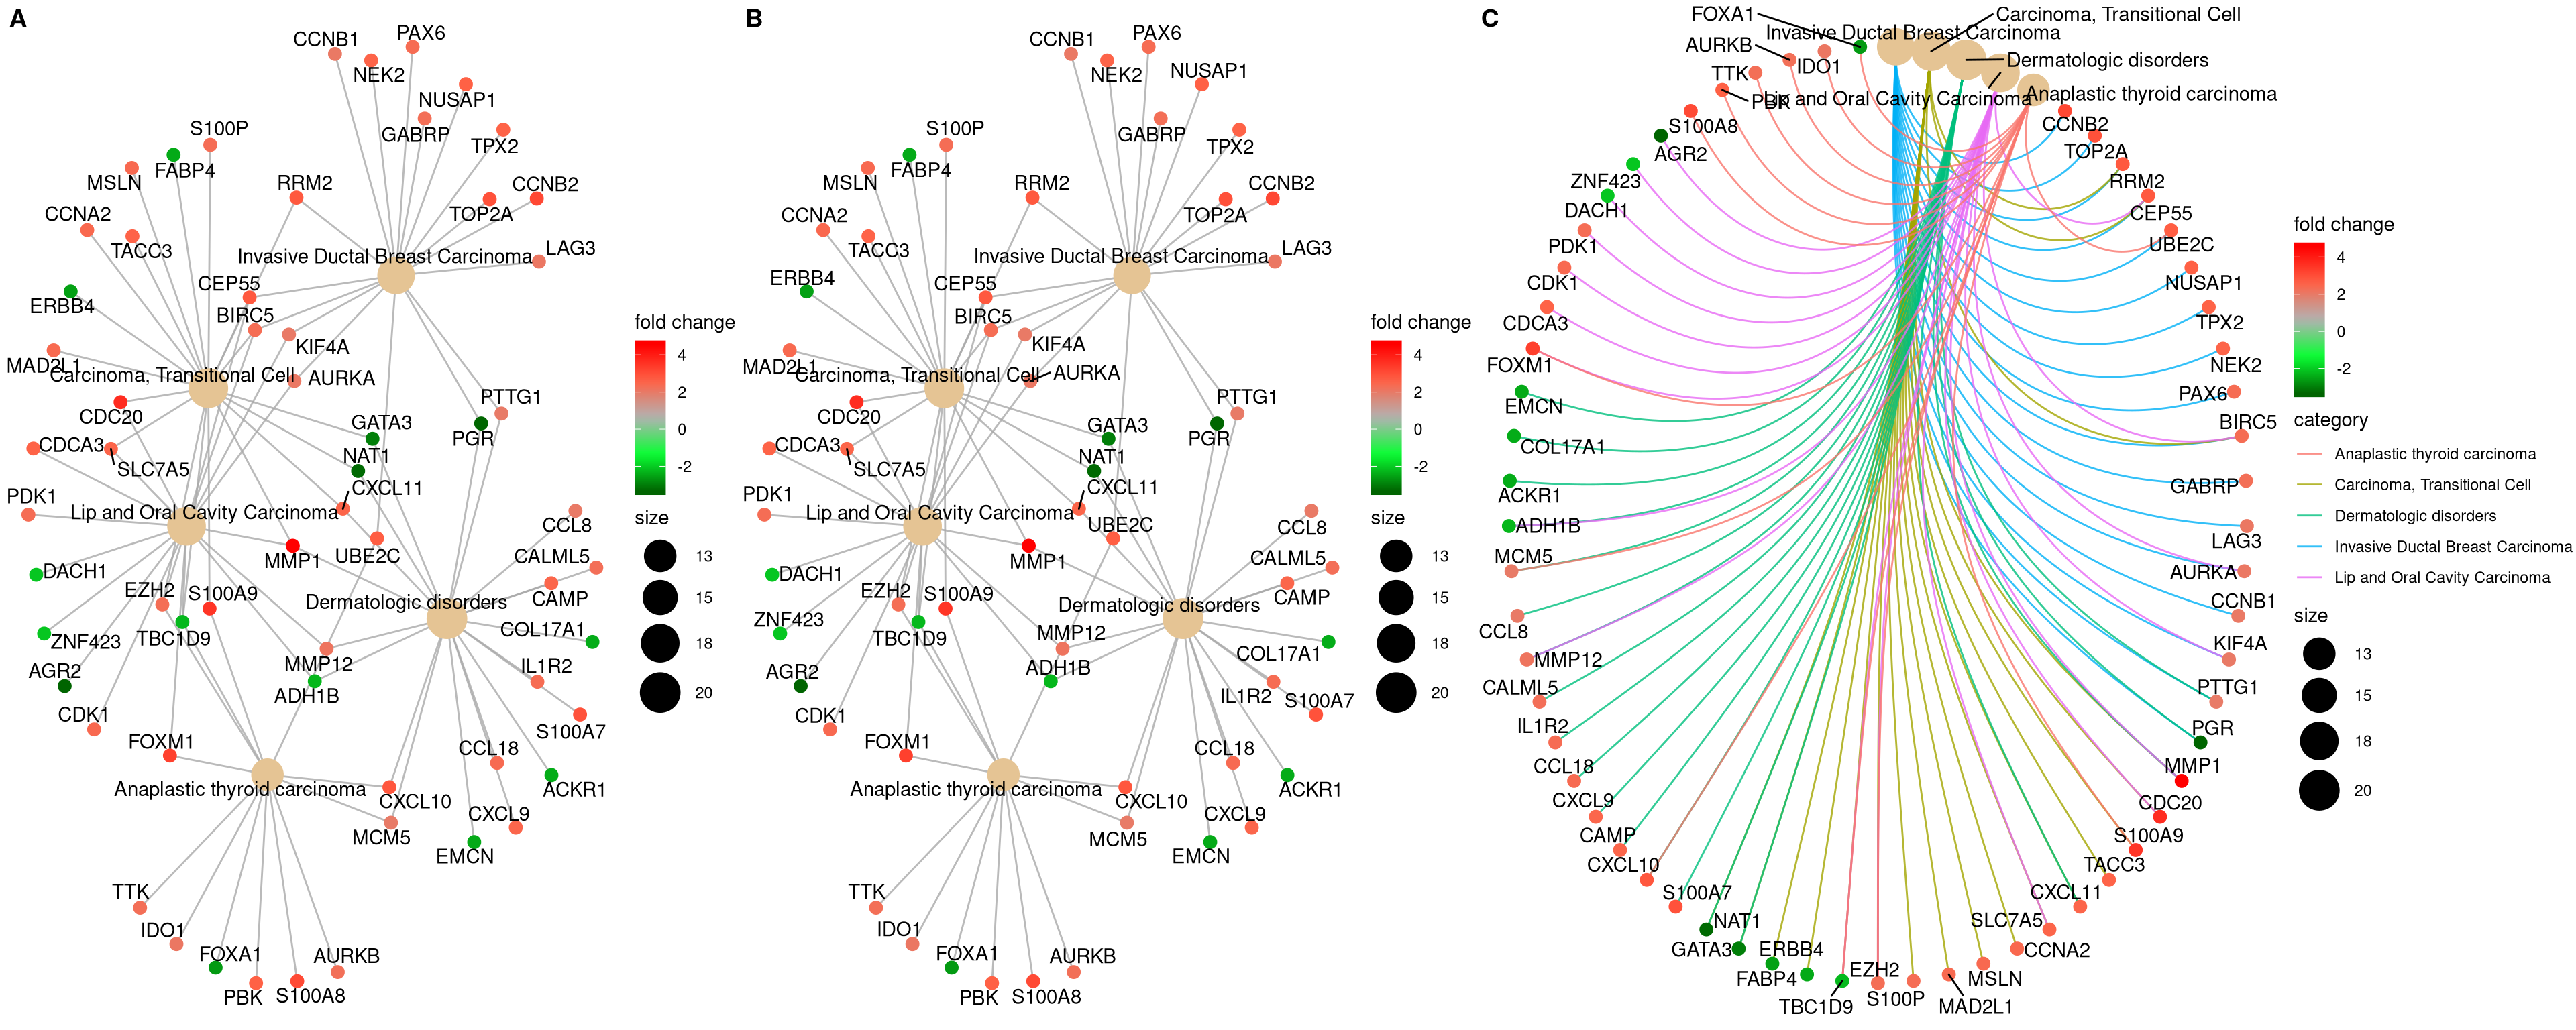
\includegraphics[width=0.8\textwidth]{figures/Networkplot-1.png}
	\end{center}
	
\blfootnote{Image taken from clusterProfiler vignette \url{https://yulab-smu.github.io/clusterProfiler-book/chapter12.html}}

\end{frame}

\begin{frame}{GO Visualisations}

	\begin{center}
	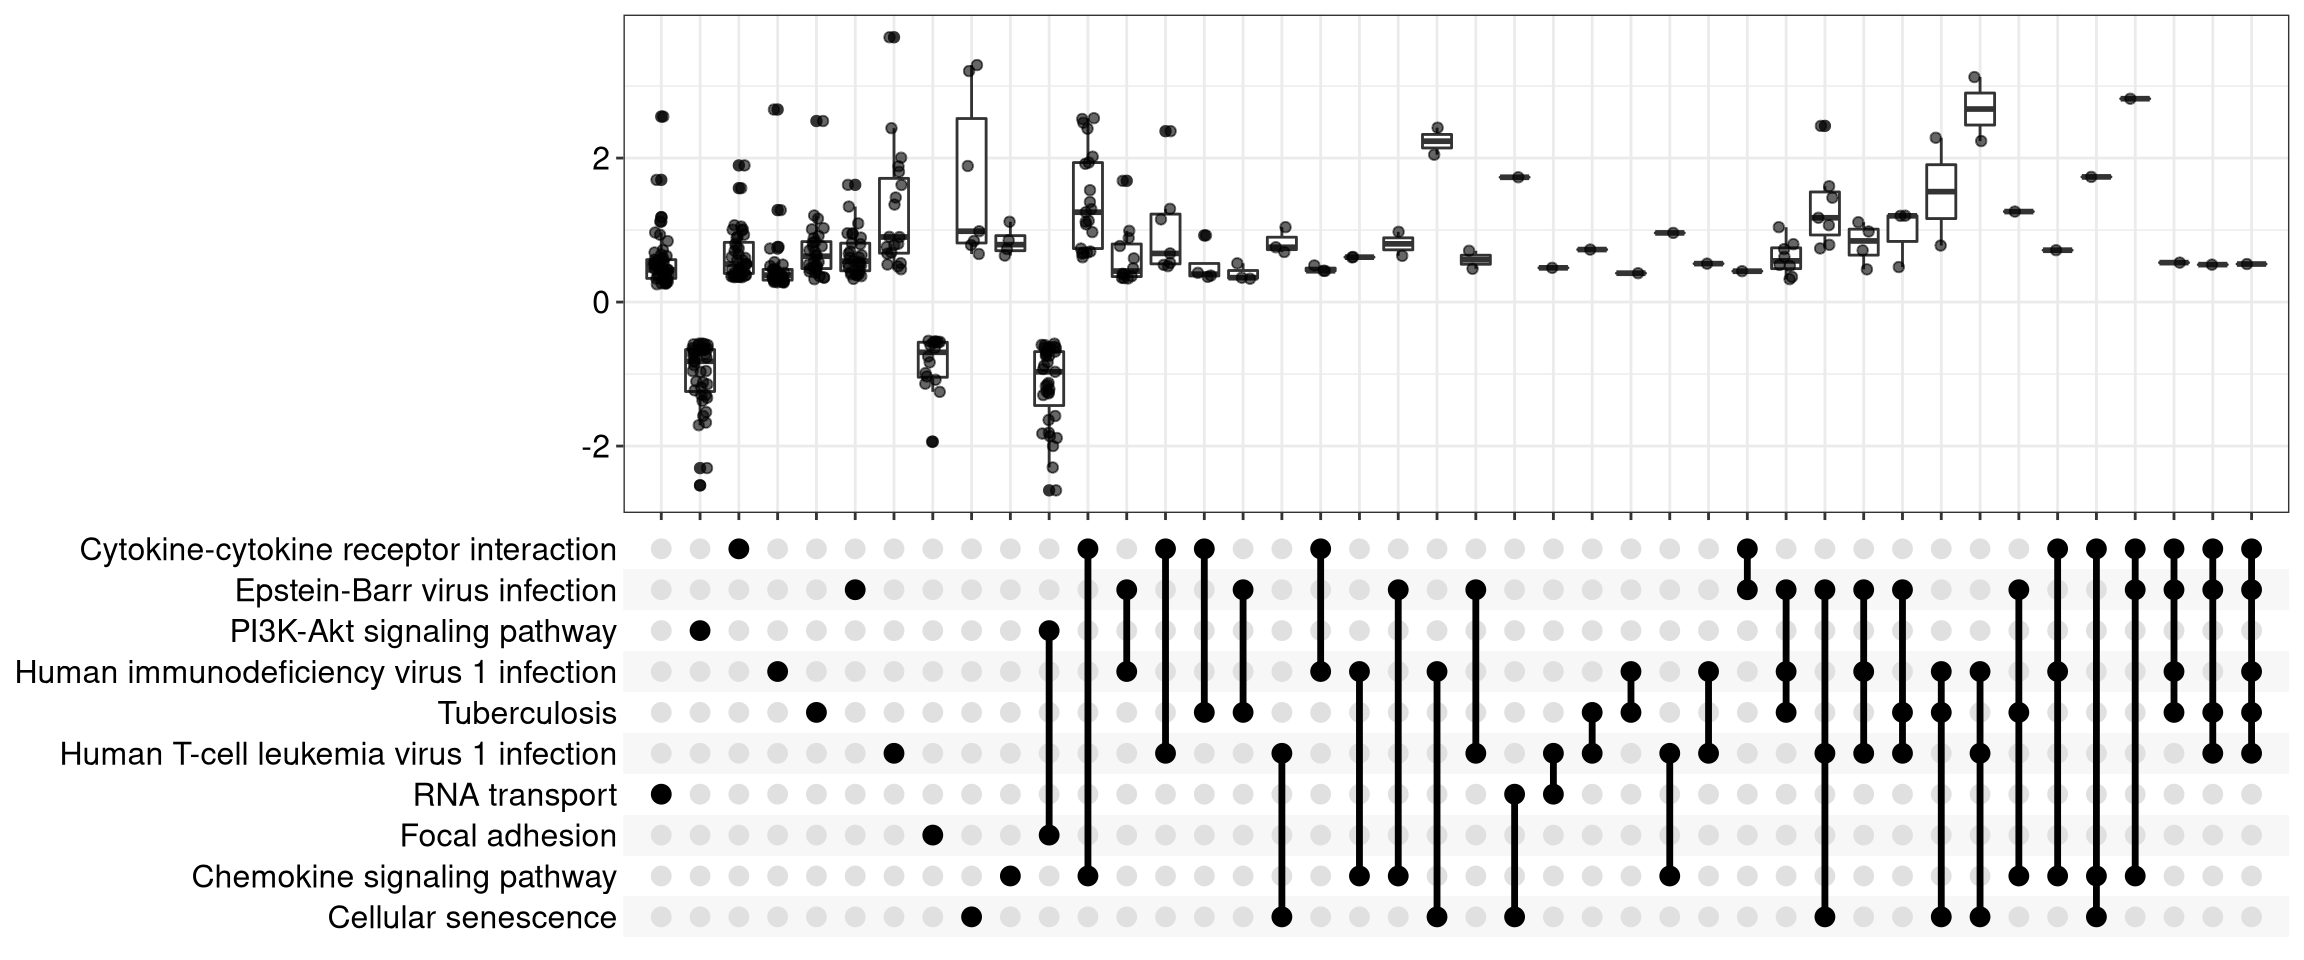
\includegraphics[width=0.8\textwidth]{figures/upsetGSEA-1.png}
	\end{center}
	
\blfootnote{Image taken from clusterProfiler vignette \url{https://yulab-smu.github.io/clusterProfiler-book/chapter12.html}}

\end{frame}

%\subsection{KEGG}

\begin{frame}{KEGG Pathways}

	\begin{itemize}
		\item The Kyoto Encyclopedia of Genes and Genomes: \textit{KEGG}
		\item KEGG Pathways are \textit{manually drawn pathway maps representing our knowledge on the molecular interaction, reaction and relation networks for}\footnote{Taken from \url{https://www.genome.jp/kegg/pathway.html}}:
		\begin{enumerate}
			\item Metabolism
			\item Genetic Information Processing
			\item Environmental Information Processing
			\item Cellular Processes
			\item Organismal Systems
			\item Human Diseases
			\item Drug Development
		\end{enumerate}
	\end{itemize}

\end{frame}

\begin{frame}{KEGG Pathways}

	\begin{itemize}
		\item Each pathway is considered as a discrete unit $\implies$ no inheritance structure
		\item Pathways may strongly overlap still: \url{https://www.genome.jp/kegg-bin/show_pathway?map01100}
		\item Can search by compounds, genes, pathways
	\end{itemize}
	
	
\end{frame}

\begin{frame}{KEGG Pathways}

	\begin{center}
	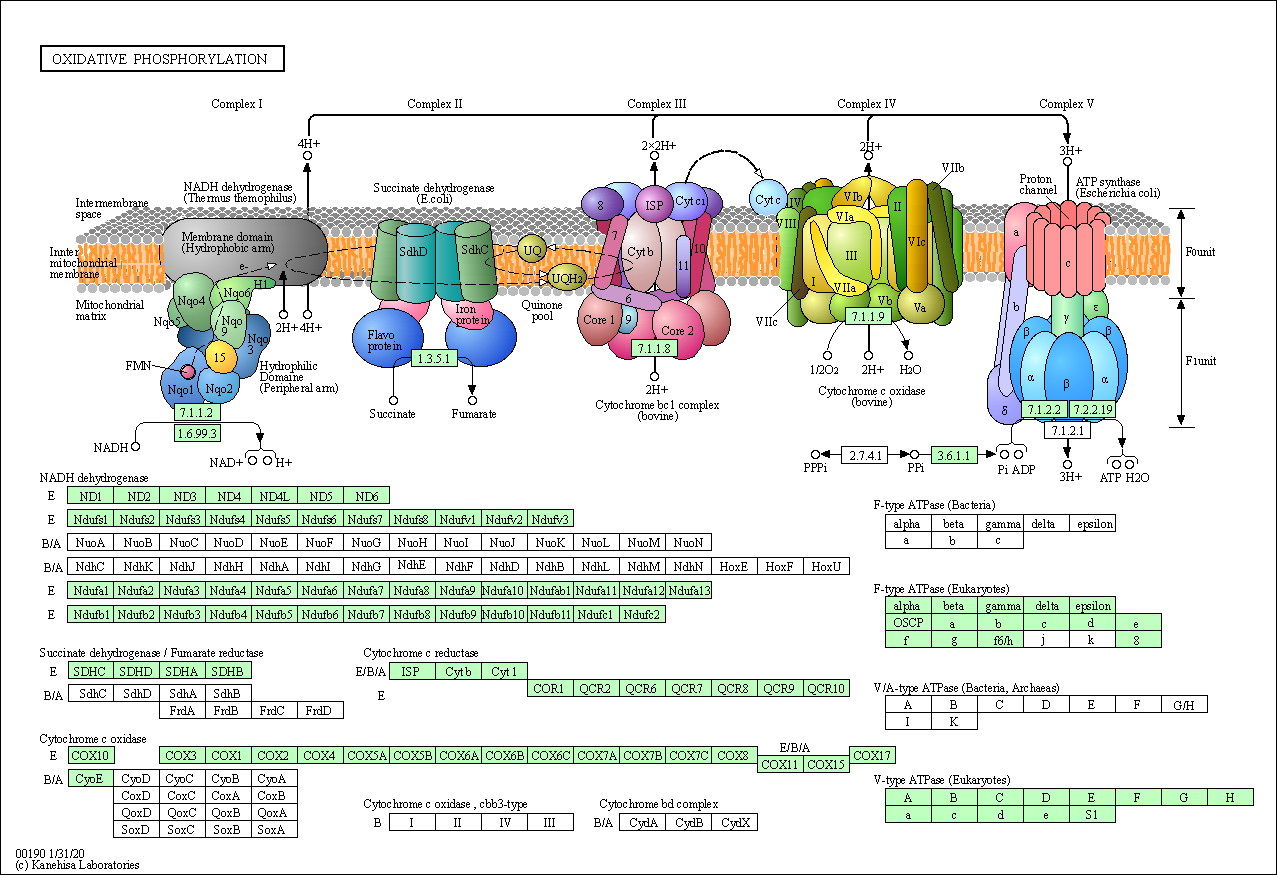
\includegraphics[width=0.6\textwidth]{figures/hsa00190.png} 
	\end{center}
	
	\blfootnote{Image downloaded from \href{https://www.genome.jp/kegg-bin/show_pathway?org_name=hsa&mapno=00190&scale=&orgs=&auto_image=&nocolor=&show_description=show}{KEGG}}

\end{frame}


\begin{frame}{KEGG Pathways}

	\begin{center}
		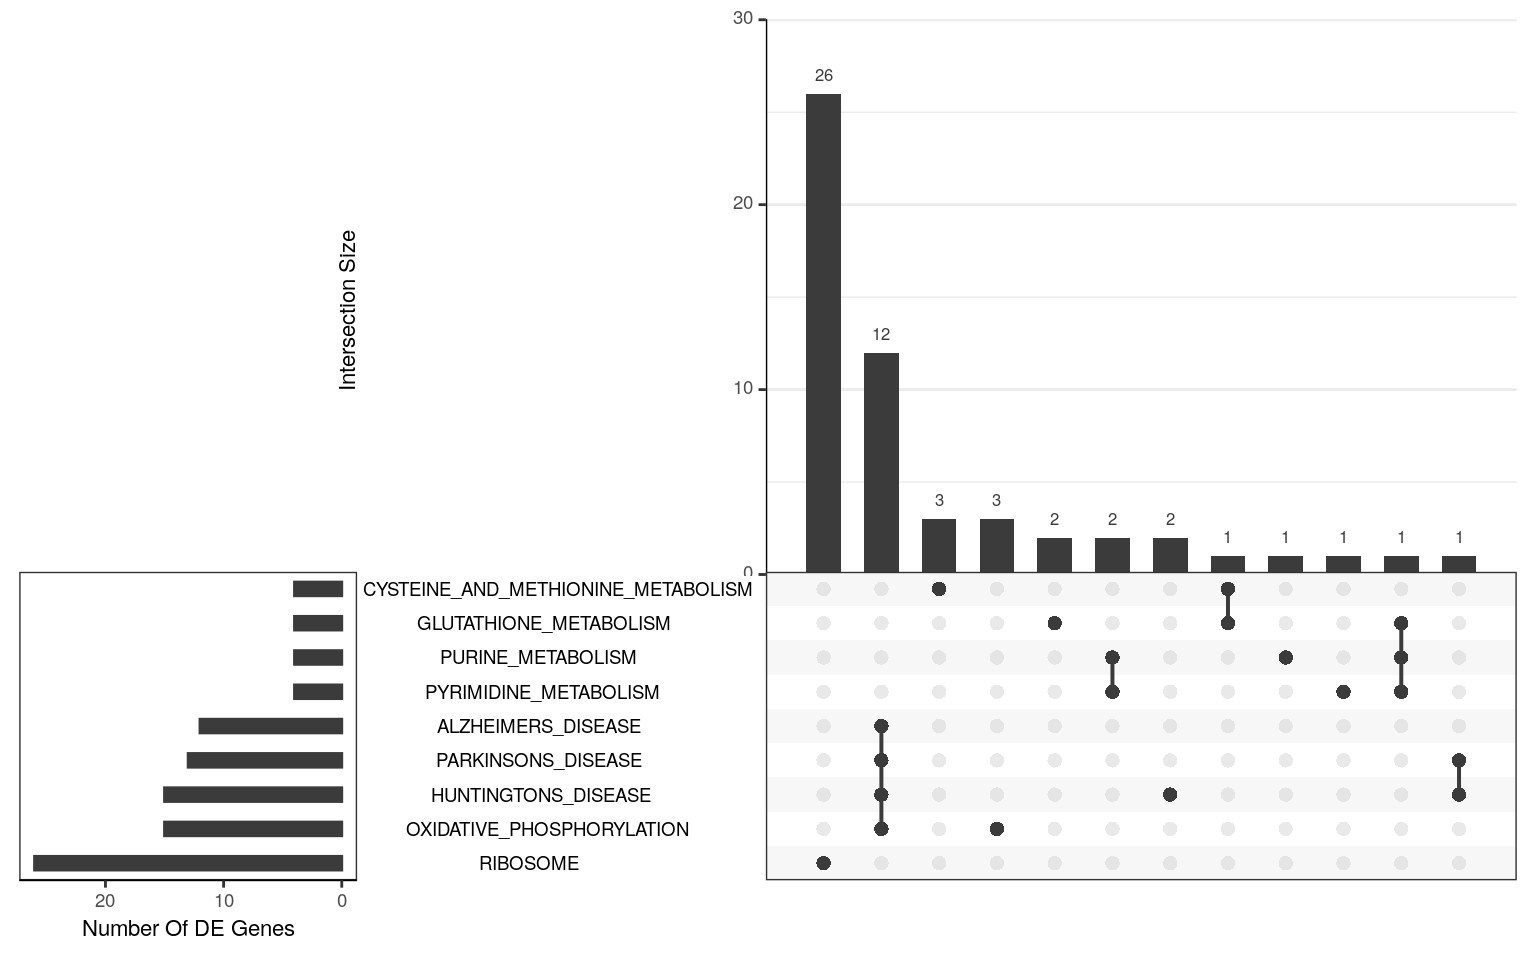
\includegraphics[width=0.7\textwidth]{figures/kgFryUpset-1.png} 
	\end{center}

\end{frame}

%\subsection{Wiki Pathways}

\begin{frame}{Wiki Pathways}

	\begin{itemize}
		\item Wiki Pathways is \textit{maintained by and for the scientific community}
		\item Not dissimilar to a a publicly maintained KEGG
		\item Currently holds 2862 pathways
	\end{itemize}

\end{frame}

\begin{frame}{Wiki Pathways}

	\begin{center}
	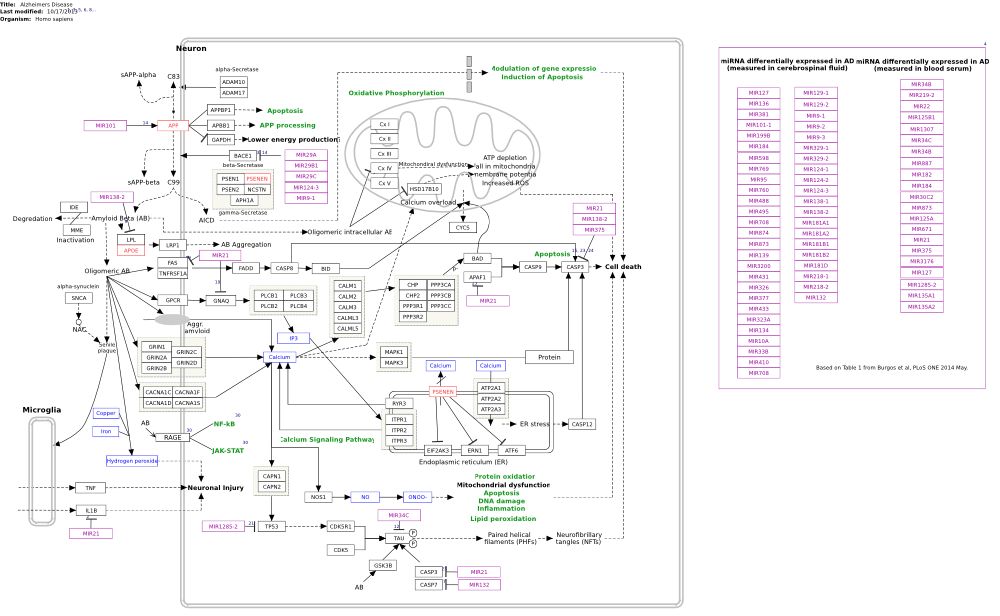
\includegraphics[width=0.6\textwidth]{figures/WP2059_108233.png} 
	\end{center}
	
	\blfootnote{Image taken from \url{https://www.wikipathways.org/index.php/Pathway:WP2059}}

\end{frame}

%\subsection{MSigDB}

\begin{frame}{The Molecular Signatures Database}

	\begin{itemize}
		\item The Molecular Signatures Database (MSigDB) collects other databases
		\begin{itemize}
			\item H: Hallmark Gene Sets
			\item C1: Positional Gene Sets
			\item C2: Curated Gene Sets (\textit{BioCarta, KEGG, Reactome})
			\item C3: Regulatory Target Gene Sets (\textit{miRNA targets, Transcription Factor targets})
			\item C4: Computational Gene Sets
			\item C5: GO Gene Sets
			\item C6: Oncogenic Gene Sets
			\item C7: Immunologic Gene Sets
		\end{itemize}
	\end{itemize}

\end{frame}

\begin{frame}{The Molecular Signatures Database}

	\begin{itemize}
		\item Doesn't use or retain identifiers from original source
		\item Datasets are supplied as \textit{species-specific} gene sets
		\item Huge redundancy
		\item Plays very nicely with R (\texttt{msigdbr})
	\end{itemize}

\end{frame}

%\subsection{Transcription Factors}

\begin{frame}{Transcription Factors}

	\begin{itemize}
		\item Transcription factors present their own unique problems
		\item Genomic binding sites allow for significant flexibility
	\end{itemize}

\end{frame}

\begin{frame}{Binding Sites}

\begin{figure}
\centering
\begin{subfigure}{.33\textwidth}
  \centering
  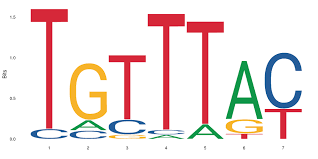
\includegraphics[width=.8\linewidth]{figures/foxp3Motif.png}
  \caption{FOXP3}
  \label{fig:sub1}
\end{subfigure}%
\begin{subfigure}{.33\textwidth}
  \centering
  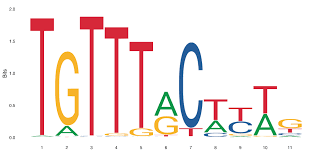
\includegraphics[width=.8\linewidth]{figures/foxa1.png}
  \caption{FOXA1}
  \label{fig:sub2}
\end{subfigure}
\begin{subfigure}{.33\textwidth}
  \centering
  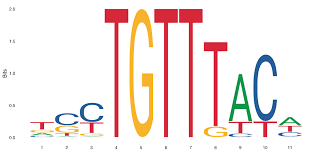
\includegraphics[width=.8\linewidth]{figures/foxo1.png}
  \caption{FOXO1}
  \label{fig:sub3}
\end{subfigure}

\label{fig:test}
\end{figure}

\end{frame}

\begin{frame}{Transcription Factors}

	\begin{itemize}
		\item Transcription factors present their own unique problems
		\item Genomic binding sites allow for significant flexibility
		\item DNA Shape can also play a role in specificity
		\item There is no 100\% match giving a binary Yes/No
		\pause
		\begin{itemize}
			\item How do we define the presence of a motif?
			\item How do we know which TF binds the motif?
			\item Does only one TF bind a genomic locus?
			\item How do we define a promoter \& which gene(s) does an enhancer influence?
		\end{itemize}
	\end{itemize}

\end{frame}

\section{Testing Within DE Genes}

\begin{frame}{Testing Our Data}

	\begin{itemize}
		\item The most common test is for enrichment of a \textit{pre-defined gene-set} within an \textit{analytically defined gene-set}
		\item Our analytically defined geneset could be:
		\begin{itemize}
			\item DE genes from a two-way comparison
			\item Some other group defining a pattern of expression
		\end{itemize}		
		\item Groups can be defined directionally or not
		\item We usually test for enrichment \textit{in comparison to a reference set of genes}
	\end{itemize}

\end{frame}

\begin{frame}{Testing Our Data}

	\begin{itemize}
		\item The most common test is \textit{Fisher's Exact Test}
		\item Tests $H_0$: \textit{No association between groups}
		\item A common reference set of genes is \textit{expressed but not DE} genes
		\item Far better than a random genomic reference
		\begin{itemize}
			\item e.g. In brain cells we compare DE in brain against expressed in brain but not DE.
			This avoids finding enrichment for ``brain-expressed genes"
		\end{itemize}
		\item Is often referred to as a \textit{hypergeometric} test
	\end{itemize}
	
\end{frame}

\begin{frame}{Testing Our Data}

An Example

	\begin{center}
		\begin{tabular}{r|rr}
			& DE & notDE \\
			\toprule
		In gene-set & 50 & 50 \\
		Not in gene-set & 950 & 15000 \\
		\midrule
		Total & 1000 & 15050 \\
		\bottomrule
		\end{tabular}
	\end{center}
	~\\[2mm]
	Under $H_0$ we expect $\pi = \frac{50}{15050} = 0.003$ of our DE genes to be in the gene set.\\[3mm]
	$(50 + 950)\times\frac{50}{15050} = 1000\times\pi = 3.32$ genes. Clearly $50 \ggg 3.32 \implies p < 2X10^{-16}$

\end{frame}

\begin{frame}{Testing Our Data}

	\begin{itemize}
		\item Fisher's Exact Test is two-sided: \textit{test is for association}
		\begin{itemize}
			\item $p_{FET} = \frac{\text{the number of more extreme tables}}{\text{the total number of possible tables}}$
		\end{itemize}
		\item Can return results which are \textbf{not} enriched
		\item Still need to use two-sided test, but can also check the observed $>$ expected
		\item Implemented in \texttt{limma} as \texttt{goana()} and \texttt{kegga()}
	\end{itemize}	
	
\end{frame}

\begin{frame}{Testing Our Data}

What about bias?

	\begin{itemize}
		\item Gene-length should be roughly constant between samples
		\item Long genes have higher counts $\implies$ biases DE
		\item Would this impact our results using Fisher's Exact Test?
		\pause
		\item \textit{Wallenius' Non-Central Hypergeometric Distribution} allows for sampling \textbf{with bias}
		\begin{itemize}
			\item Also very applicable if GC content varies across samples/groups
		\end{itemize}
		\item This incorporation of bias is implemented in \texttt{goseq}\footfullcite{pmid20132535}
	\end{itemize}	
	
\end{frame}

\begin{frame}{Testing Our Data}

	\begin{center}
		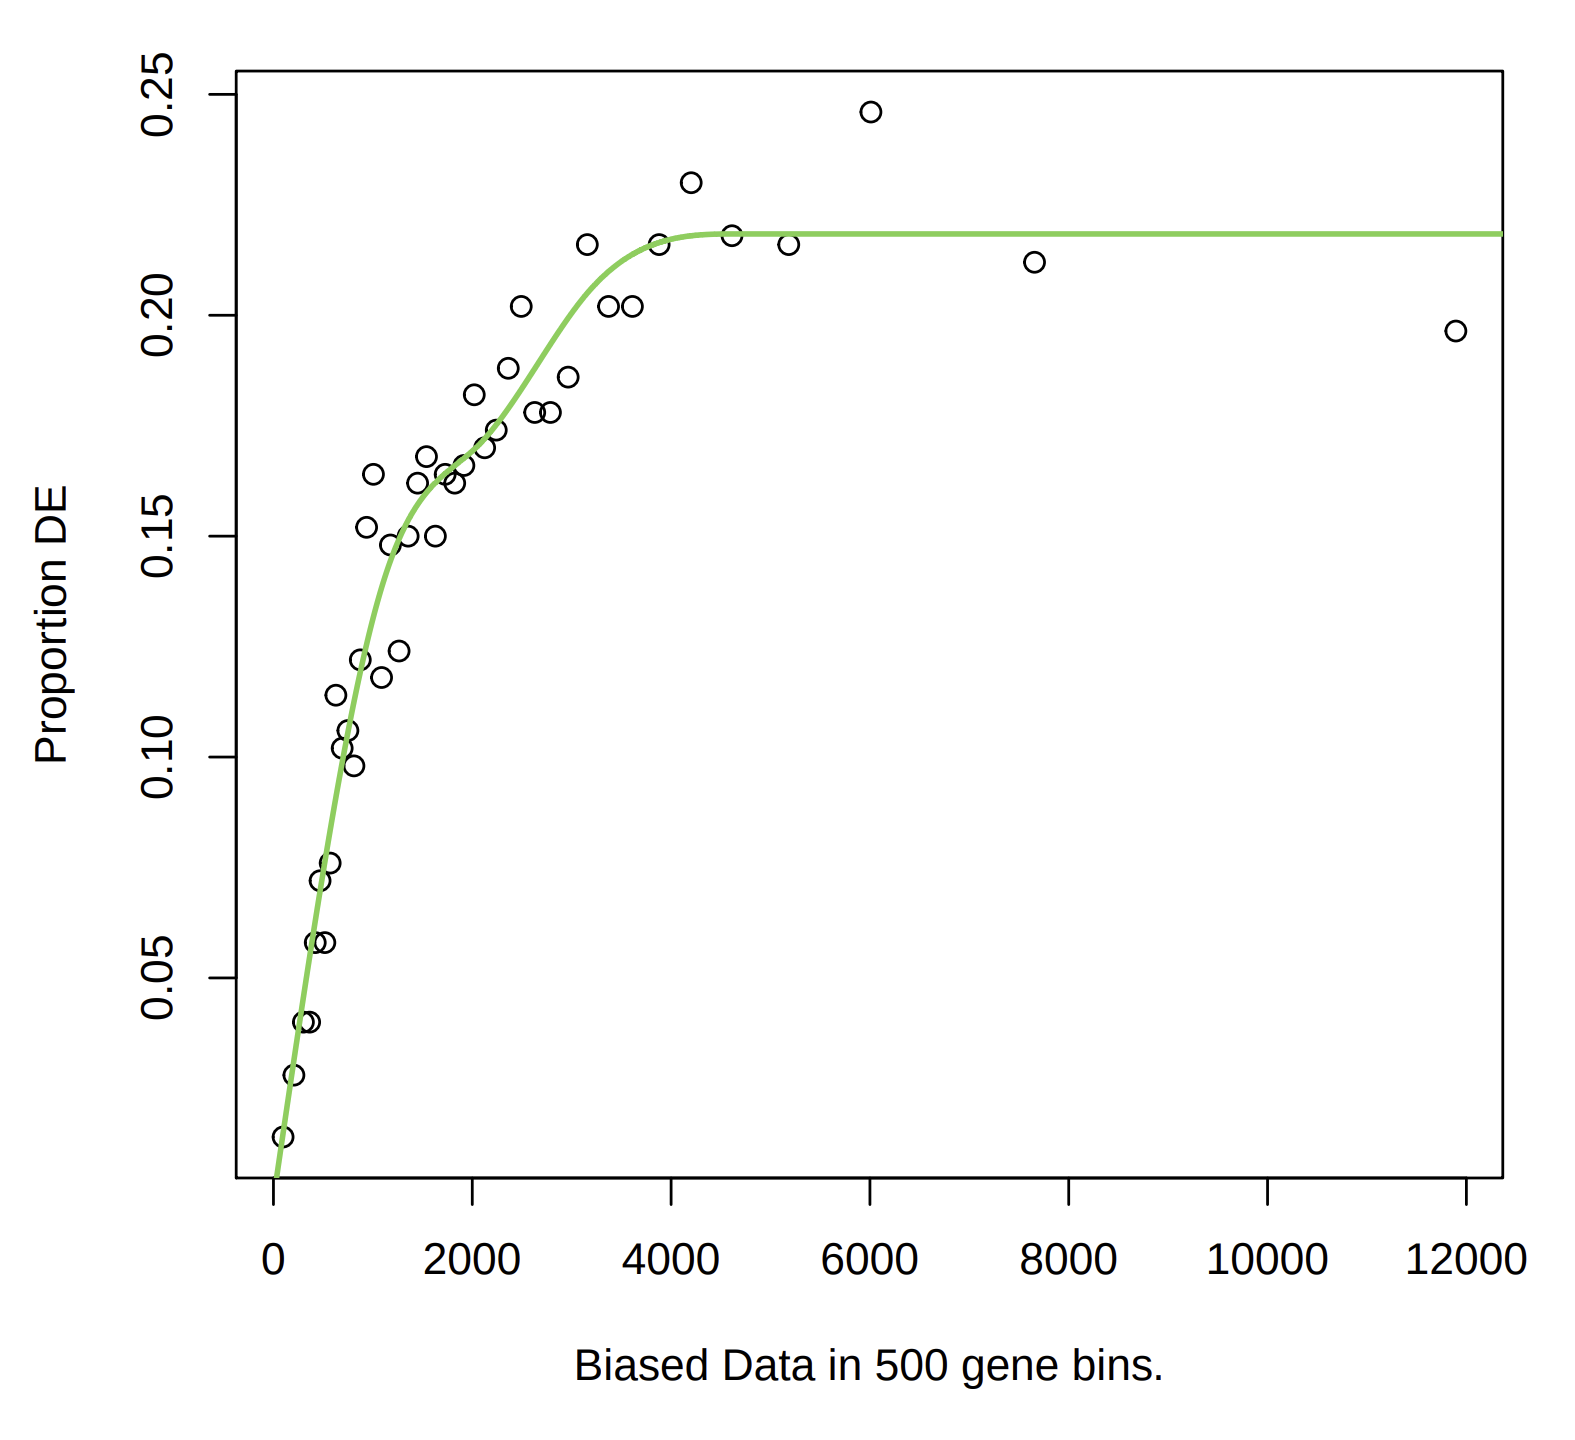
\includegraphics[width=0.47\linewidth]{figures/pwfLength.png} 
	\end{center}		
	
	\blfootnote{Taken from \url{https://bioconductor.org/packages/release/bioc/vignettes/goseq/inst/doc/goseq.pdf}}	
	
\end{frame}

\begin{frame}{Testing Our Data}

In all cases:

	\begin{enumerate}
		\item We obtain a set of analytically defined genes (e.g. DE genes)
		\item We test multiple predefined gene sets (usually 1000s)
		\item We obtain a list of results with $p$-values
		\item We adjust the $p$-values
	\end{enumerate}
	
\end{frame}

\begin{frame}{Adjusting P-Values}

	\begin{itemize}
		\item If there are no DE genes in a GO term (i.e. a gene-set), would we test for enrichment?
		\begin{itemize}
			\item We could remove these gene-sets from our gene sets to be tested
			\item Do we require a minimum number of DE genes in the gene-set to be interested?
		\end{itemize}
		\item If using GO terms, those near the Ontology root tend to be uninformative
		\begin{itemize}
			\item Remove terms based on shortest/longest path to root node?
		\end{itemize}
		\item FDR-adjustment or Bonferroni?
		\begin{itemize}
			\item Do we care more about Type I or Type II errors
			\item Under Bonferroni $p < 0.05$ is a difficult threshold to cross
		\end{itemize}
	\end{itemize}
	
\end{frame}


\section{Using Ranked Lists}

\begin{frame}{Using Ranked Lists}

	\begin{itemize}
		\item All of the above looks for enrichment \textbf{within} an analytically-derived gene set
		\item This focusses on genes with the most significantly altered expression
		\item Are other biological behaviours worth exploring
		\pause
		\item What if an entire pathway is up-regulated a very small amount?
		\item We can use ranked lists to test for ``enrichment"
		\begin{itemize}
			\item We can rank on t-statistic, p-value or any appropriate statistic
		\end{itemize}
	\end{itemize}

\end{frame}

\begin{frame}{Using Ranked Lists}

	\begin{itemize}
		\item The first approach proposed for this was \textit{Gene Set Enrichment Analysis}, (GSEA)\footfullcite{Subramanian15545}
		\item ``Takes a walk" down a ranked list and increases the \textit{enrichment score} every time a gene is found from the gene-set
		\item Find the maximum deviation from zero and considers that the Enrichment Score
		\item All Enrichment Scores for a gene set are then normalised $\implies$ Normalised Enrichment Score
		\item The position \textit{up to the maximal ES} is often called the \textit{leading edge}
	\end{itemize}


\end{frame}

\begin{frame}{Using Ranked Lists}

	\begin{center}
		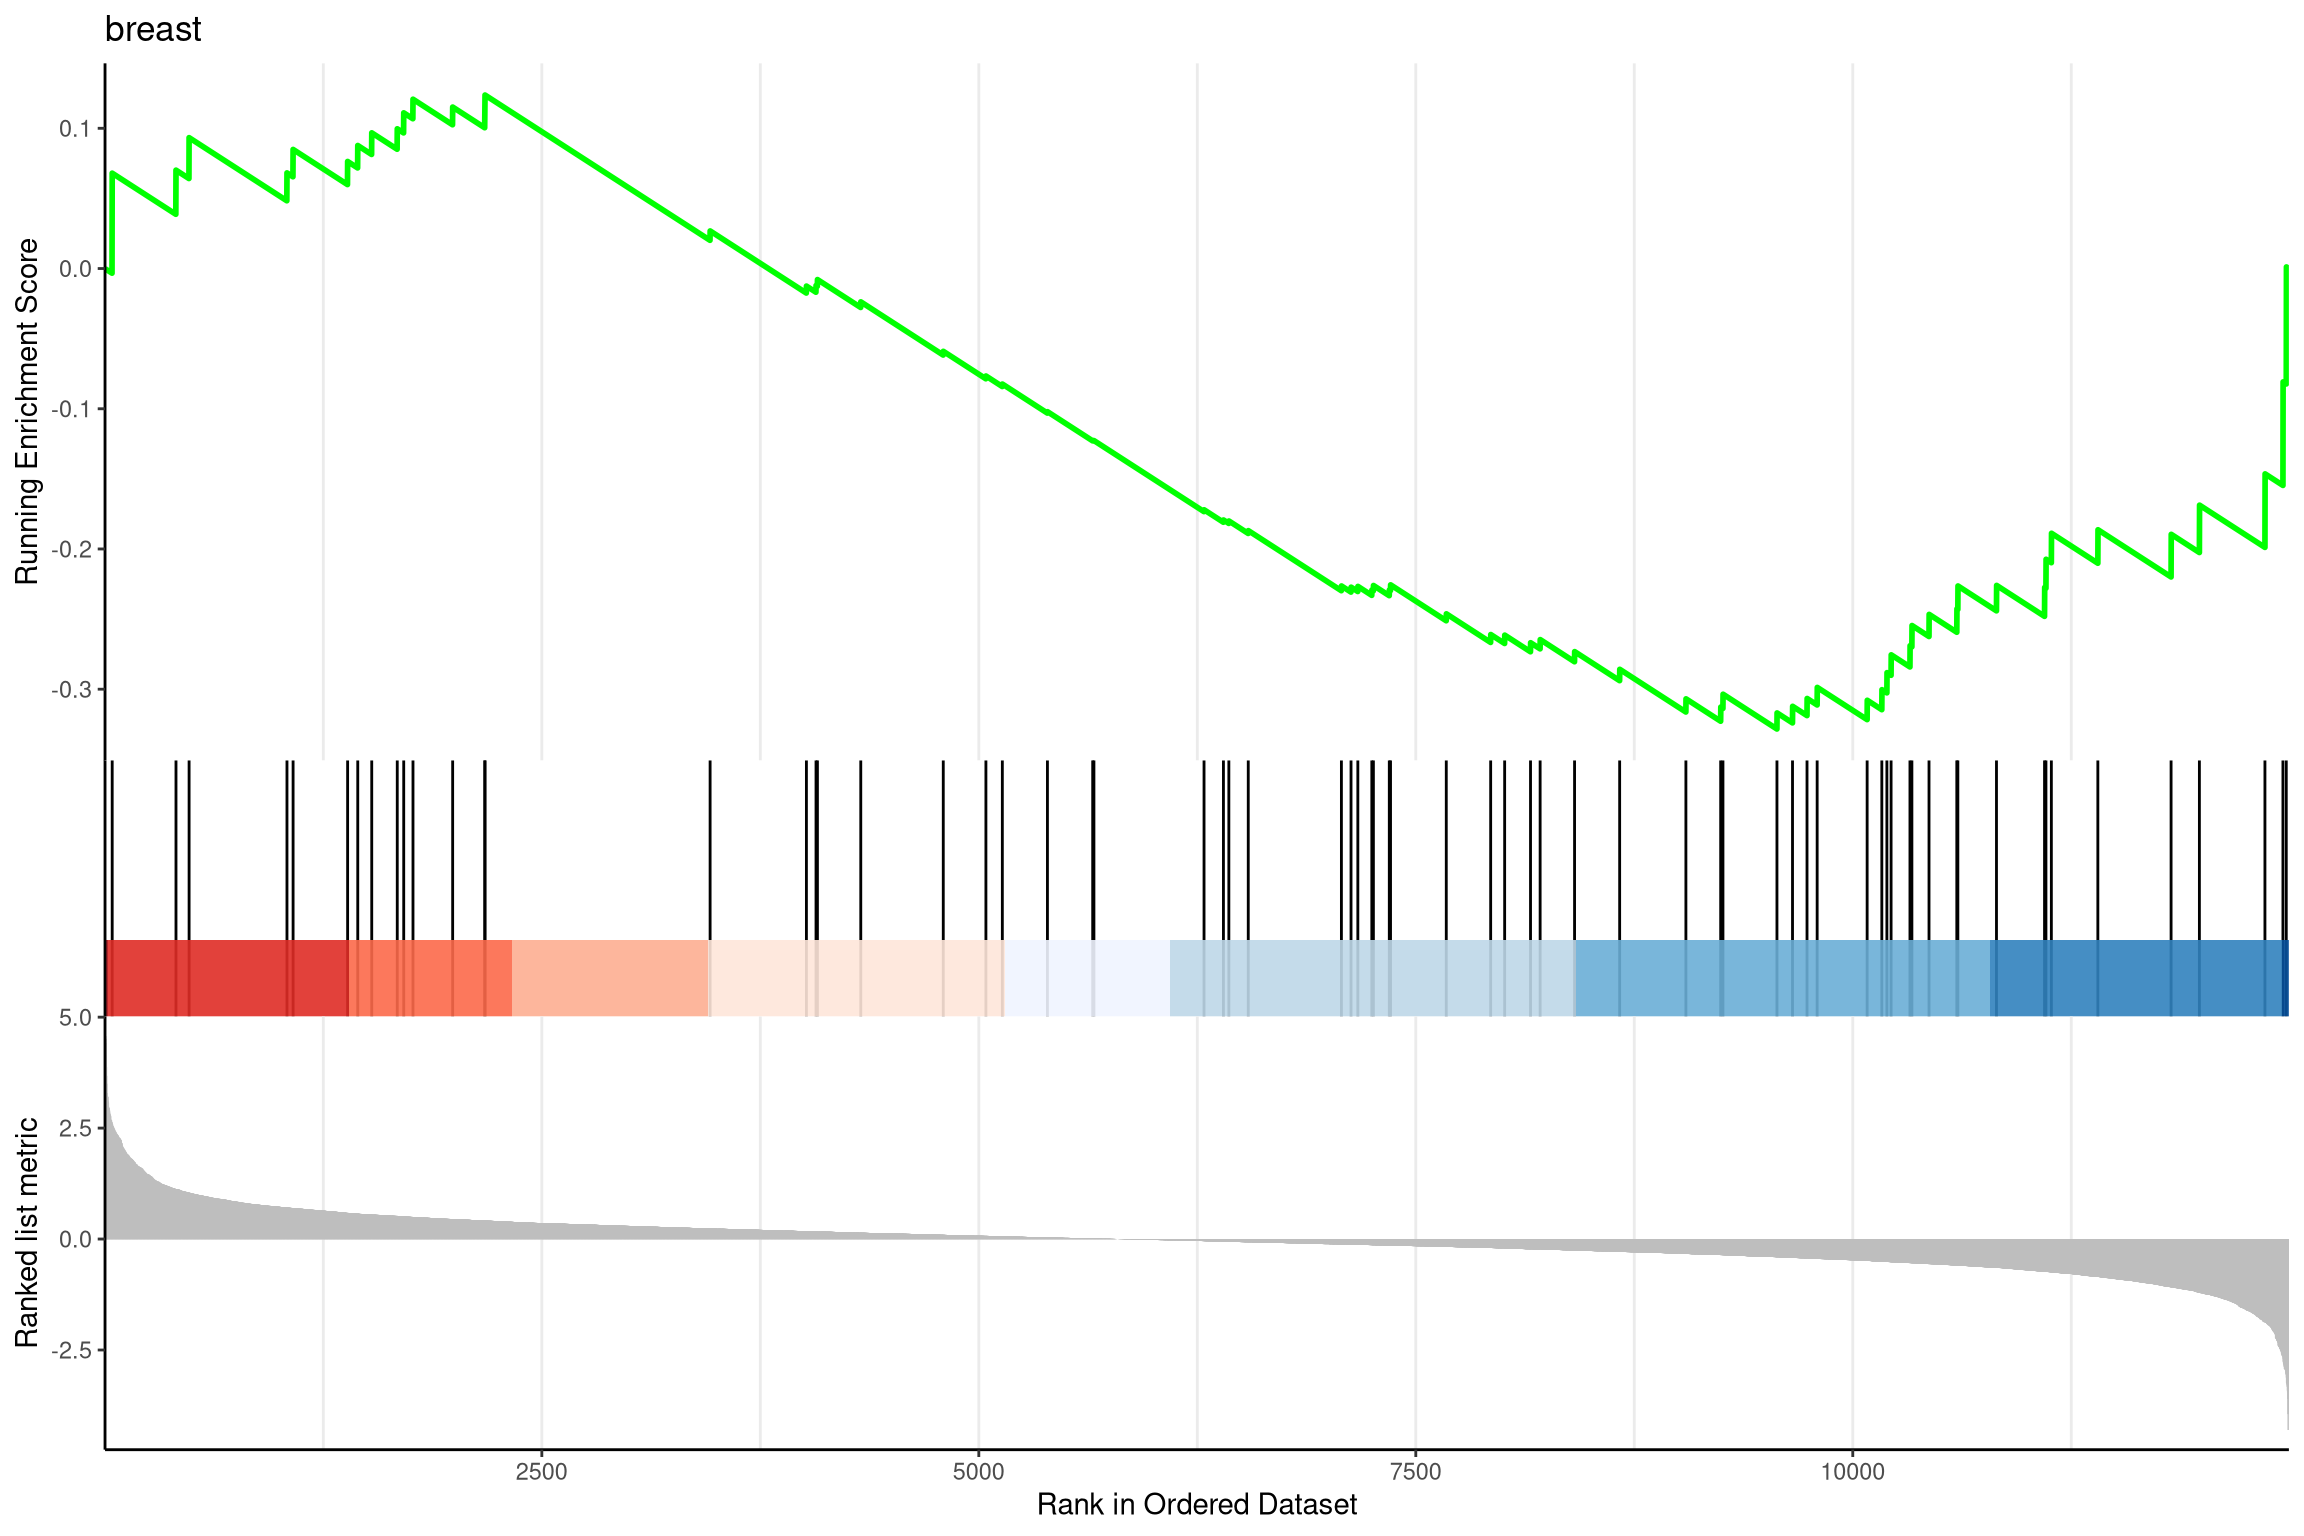
\includegraphics[width=0.5\linewidth]{figures/gseaplot2-1.png} 
	\end{center}
	
	\begin{itemize}
		\item Here, the walk began at the most \textit{downregulated} gene
		\item The leading edge would be genes to the right of the maximal ES (below the axis)
	\end{itemize}
	
	
	\blfootnote{Image taken from clusterProfiler vignette \url{https://yulab-smu.github.io/clusterProfiler-book/chapter12.html}}


\end{frame}

\begin{frame}{Using Ranked Lists}

	\begin{itemize}
		\item This approach is independent of any significantly DE genes
		\item Significance for a gene-set is obtained by comparing the ES to a Null distribution
		\begin{itemize}
			\item Null distribution is obtained by permutation of samples/genes
		\end{itemize}
		\item The end result is not dissimilar to the non-parametric Kolgorov-Smirnov test
		\item \textbf{However} this approach is very sensitive to bias and inter-gene correlations
	\end{itemize}

\end{frame}

\begin{frame}{Using Ranked Lists}

	\begin{itemize}
		\item If GC or length bias shows strong correlation with treatment groups $\implies$ lots of spurious results
	\end{itemize}
	~\\[4mm]
	\begin{center}
		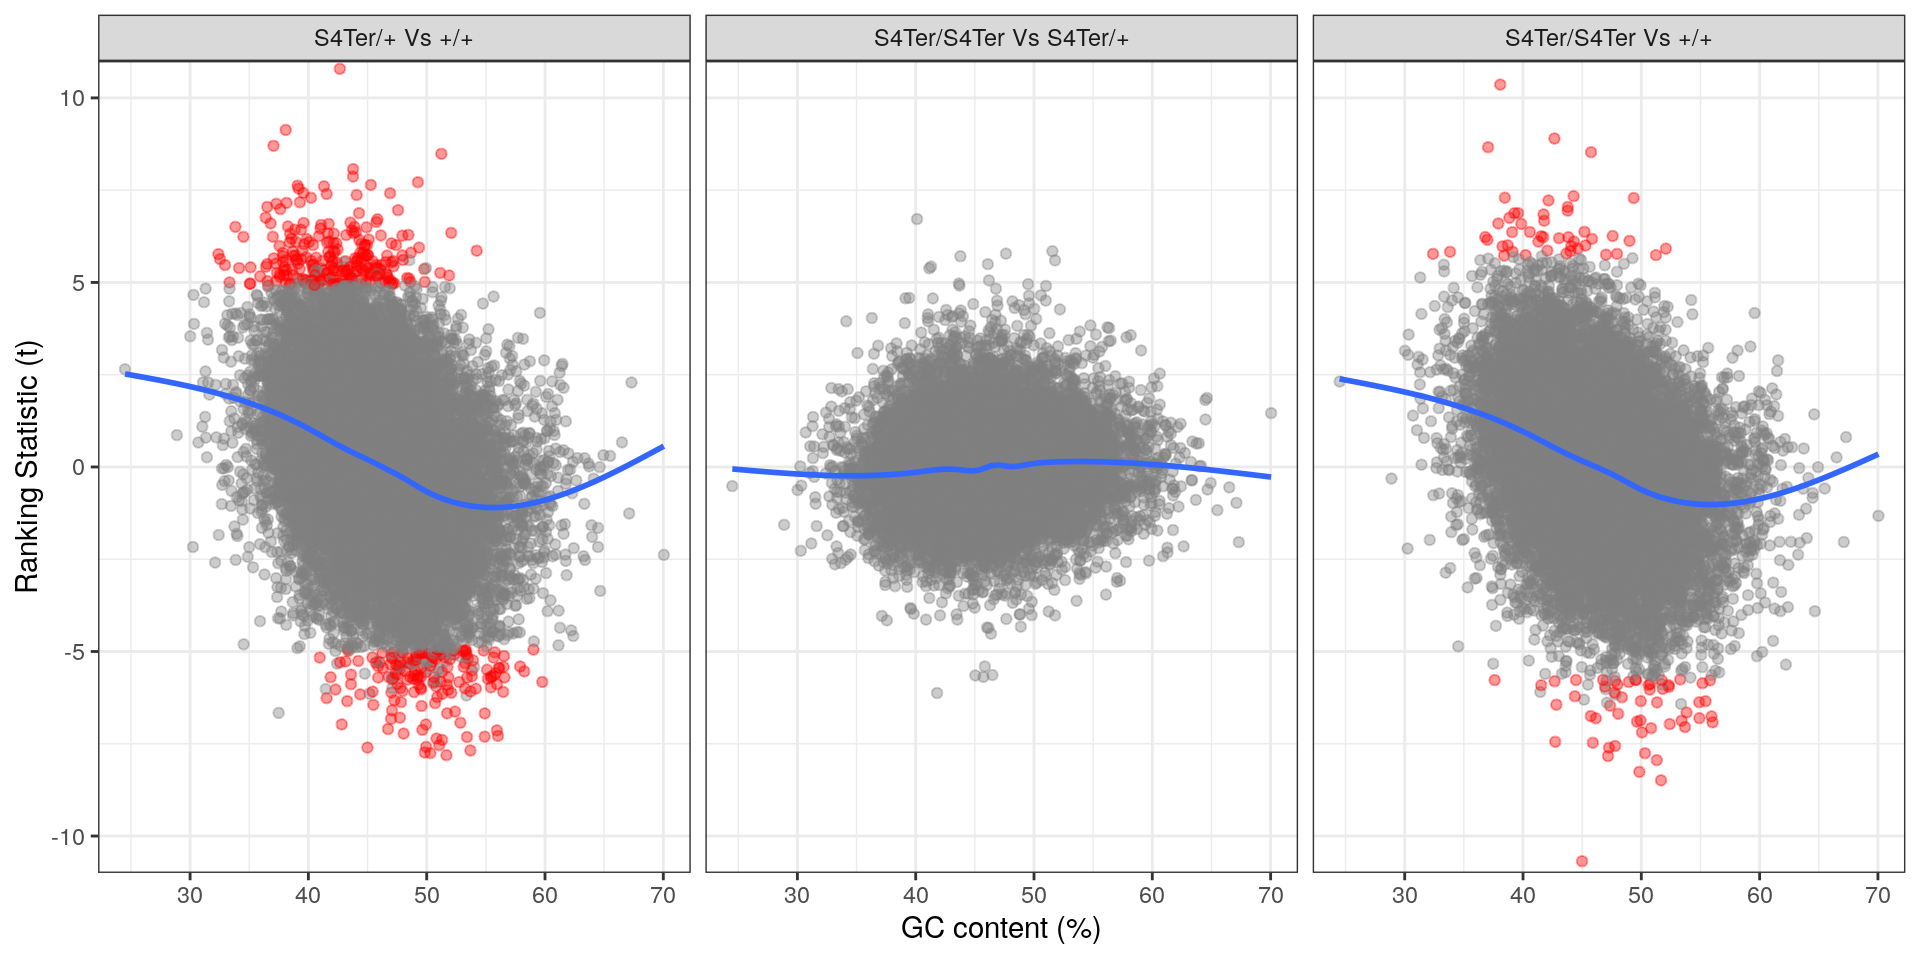
\includegraphics[width=0.6\textwidth]{figures/voomGCBias-1.png} 
	\end{center}
	
\end{frame}

\begin{frame}{Using Ranked Lists}

	\begin{itemize}
		\item An alternative is ROAST, which uses rotation testing not permutation
		\item Inter-gene correlations are \textit{explicitly accommodated}
		\item A gene-set level $T$-statistic is obtained, with a p-value by Monte-Carlo (rotation)
		\item A fast version is implemented in \texttt{limma} as \texttt{fry()}.
		\begin{itemize}
			\item No direct equivalent to the leading edge is obtained
			\item Crude approximation may be genes with $|T| > 2$
		\end{itemize}
	\end{itemize}

\end{frame}

\begin{frame}{Using Ranked Lists}

	\begin{itemize}
		\item Many alternatives exist
		\begin{itemize}
			\item Wilcoxon Rank Sum Test, Kolgorov-Smirnov
			\item Hypergeomteric testing whilst walking down a list
		\end{itemize}
		\item The package \texttt{EGSEA} integrates multiple methods
		\item We want to capture real biology \textbf{not} artefacts from bias
	\end{itemize}
	
\end{frame}

\begin{frame}{Summary}

	\begin{itemize}
		\item Testing within a set of DE genes against non-DE genes, for enrichment \textit{within} the DE genes
		\item Testing along a ranked list for enrichment at either end
		\item Multiple testing applies under both approaches $\implies$ strong biological signals only
		\item Gene-sets can be literally anything (TFBS, miR targets, KEGG pathway)
		\begin{itemize}
			\item We can also define our own gene-sets, i.e. 3'UTR with IRE
		\end{itemize}
		\item Visualisations can be very challenging
	\end{itemize}

\end{frame}




\end{document}
